\documentclass[review,1p]{elsarticle}

\usepackage{mypreamble}
%% Acronym definitions loaded before the manuscript body.

\acrodef{LCZ}{Local Climate Zone}
\acrodef{DSM}{surface model}
\acrodef{DTM}{Digital Terrain Model}
\acrodef{nDSM}{normalized surface model}
\acrodef{SVF}{Sky View Factor}
\acrodef{LST}{Land Surface Temperature}
\acrodef{NDVI}{Normalized Difference Vegetation Index}
\acrodef{NDBI}{Normalized Difference Built-up Index}
\acrodef{NDWI}{Normalized Difference Water Index}
\acrodef{GEE}{Google Earth Engine}
\acrodef{OSM}{OpenStreetMap}
\acrodef{CRS}{Coordinate Reference System}
\acrodef{FUR}{Functional Urban Region}
\acrodef{CNN}{Convolutional Neural Network}
\acrodef{ViT}{Vision Transformer}
\acrodef{MLP}{Multilayer Perceptron}
\acrodef{RF}{Random Forest}
\acrodef{SHAP}{SHapley Additive exPlanations}
\acrodef{XAI}{Explainable Artificial Intelligence}
\acrodef{CV}{Cross-Validation}
\acrodef{MAUP}{Modifiable Areal Unit Problem}
\acrodef{ARI}{Adjusted Rand Index}
\acrodef{F1}{F1-score}
\acrodef{MCC}{Matthews Correlation Coefficient}
\acrodef{RMSE}{Root Mean Square Error}
\acrodef{MAE}{Mean Absolute Error}


\journal{Sustainable Cities and Society}

\begin{document}

\graphicspath{{../../figures/main/}{../../figures/supplementary/}}

\begin{frontmatter}
\title{Supplementary material for: Climorfa: Climate-Sensitive Urban Morphology in Izmir}
\author{Author information removed for double-anonymized review}
\end{frontmatter}

\renewcommand{\thefigure}{S\arabic{figure}}
\setcounter{figure}{0}

\section*{Supplementary diagnostics and reproducibility evidence}

This reconstructed supplement contains the current evidence-bearing bundle
identified in the project figure map. It is deliberately limited to diagnostics
that support interpretation of the weak-label baseline and reproducibility. It
does not contain retired external-triangulation diagnostics, duplicate
weak-label panels, or untrained deep-model outputs.

\subsection*{S1. Matched urban-texture, surface-model, and canopy atlas}

The atlas contains the same 48 deterministic selection cells used for the
within-class climate--morphology comparison. Each cell is shown through matched
figure-ground texture, surface-model elevation/roughness, and cleaned 10 m
canopy-height views. Rows separate the lower and upper within-class summer-LST
quartiles; columns represent deterministic prototype rules. The atlas is
descriptive and reproducible from the exported selection manifest, not an
audited local subtype validation.

\begin{figure*}[p]
    \centering
    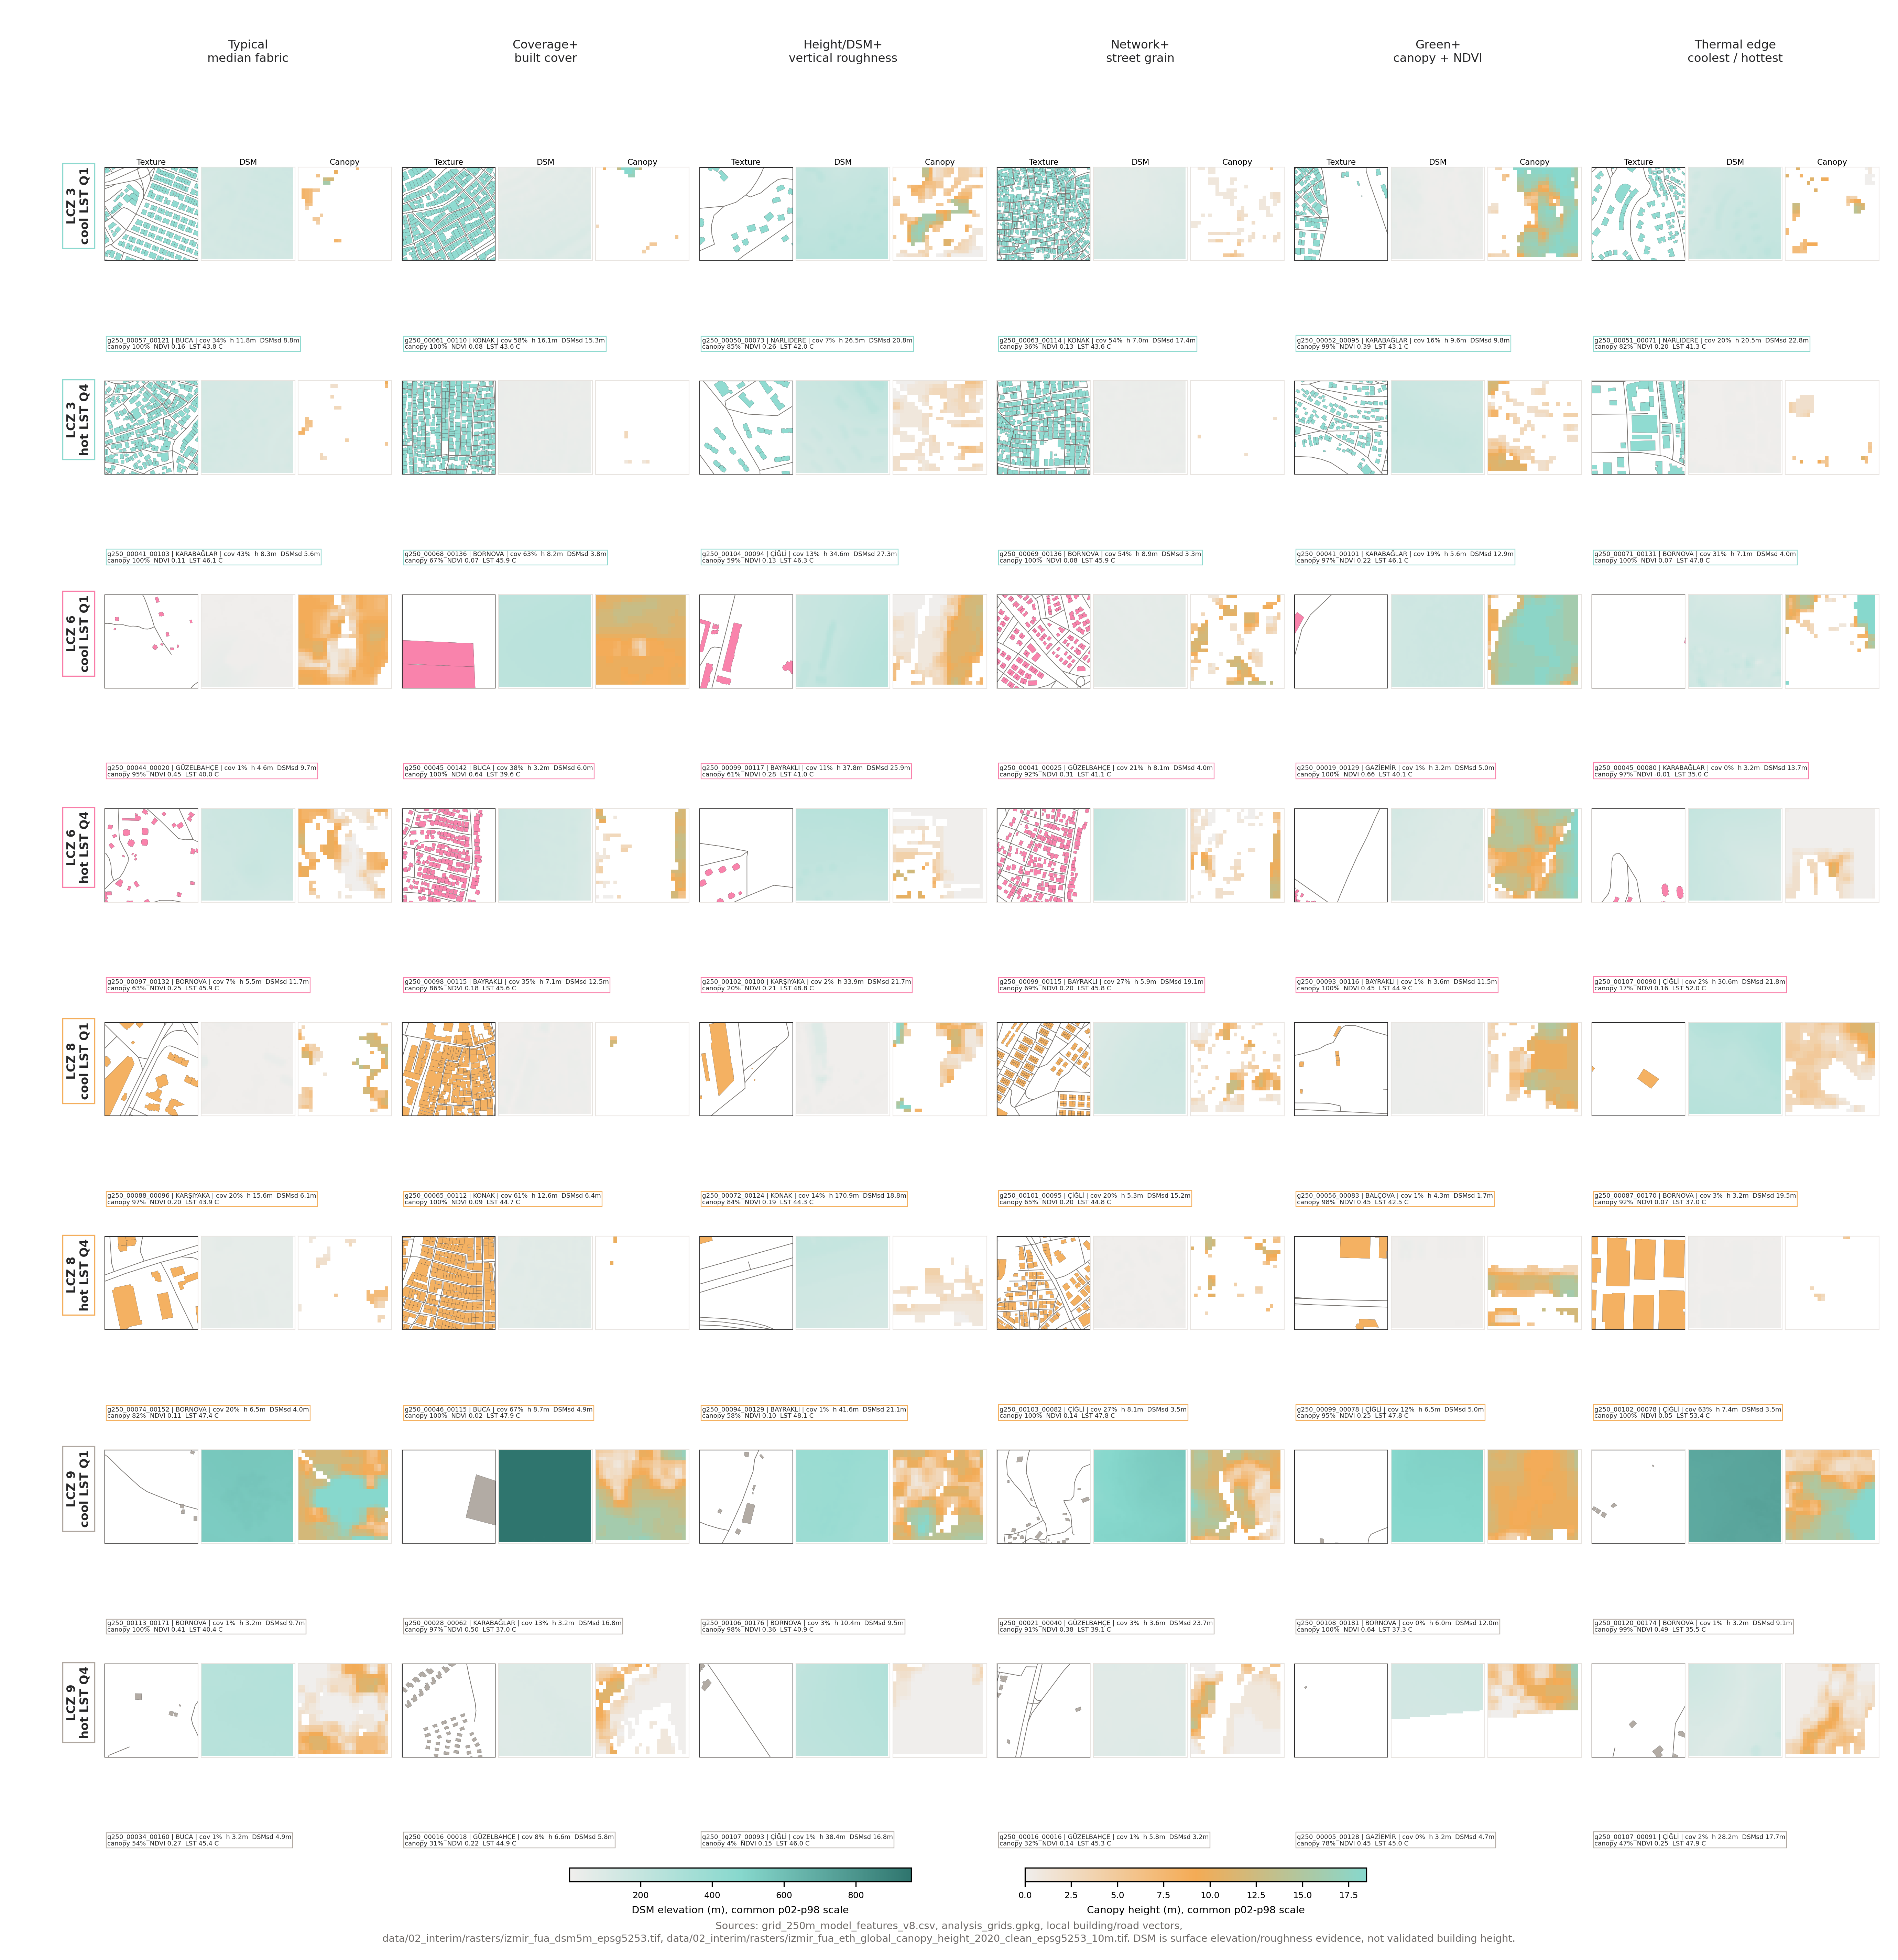
\includegraphics[width=\textwidth]{fig_s1_texture_dsm_canopy_atlas_48_cells.png}
    \caption{Matched 48-cell urban-texture atlas. Each selected cell contains
    figure-ground texture, surface-model elevation/roughness, and canopy-height
    views on shared robust scales. The figure is a visual evidence bridge, not
    a validated building-height or audited local-classification result.}
    \label{fig:s1-texture-surface-canopy}
\end{figure*}
\FloatBarrier

\subsection*{S2. Feature quality and collinearity}

Feature missingness is interpreted together with structural-absence flags before
fold-specific imputation. The collinearity panel records the largest groups at
absolute correlation $r\geq0.95$; family-level ablations and representative
variables are used to reduce redundancy in the reported baselines.

\begin{figure*}[p]
    \centering
    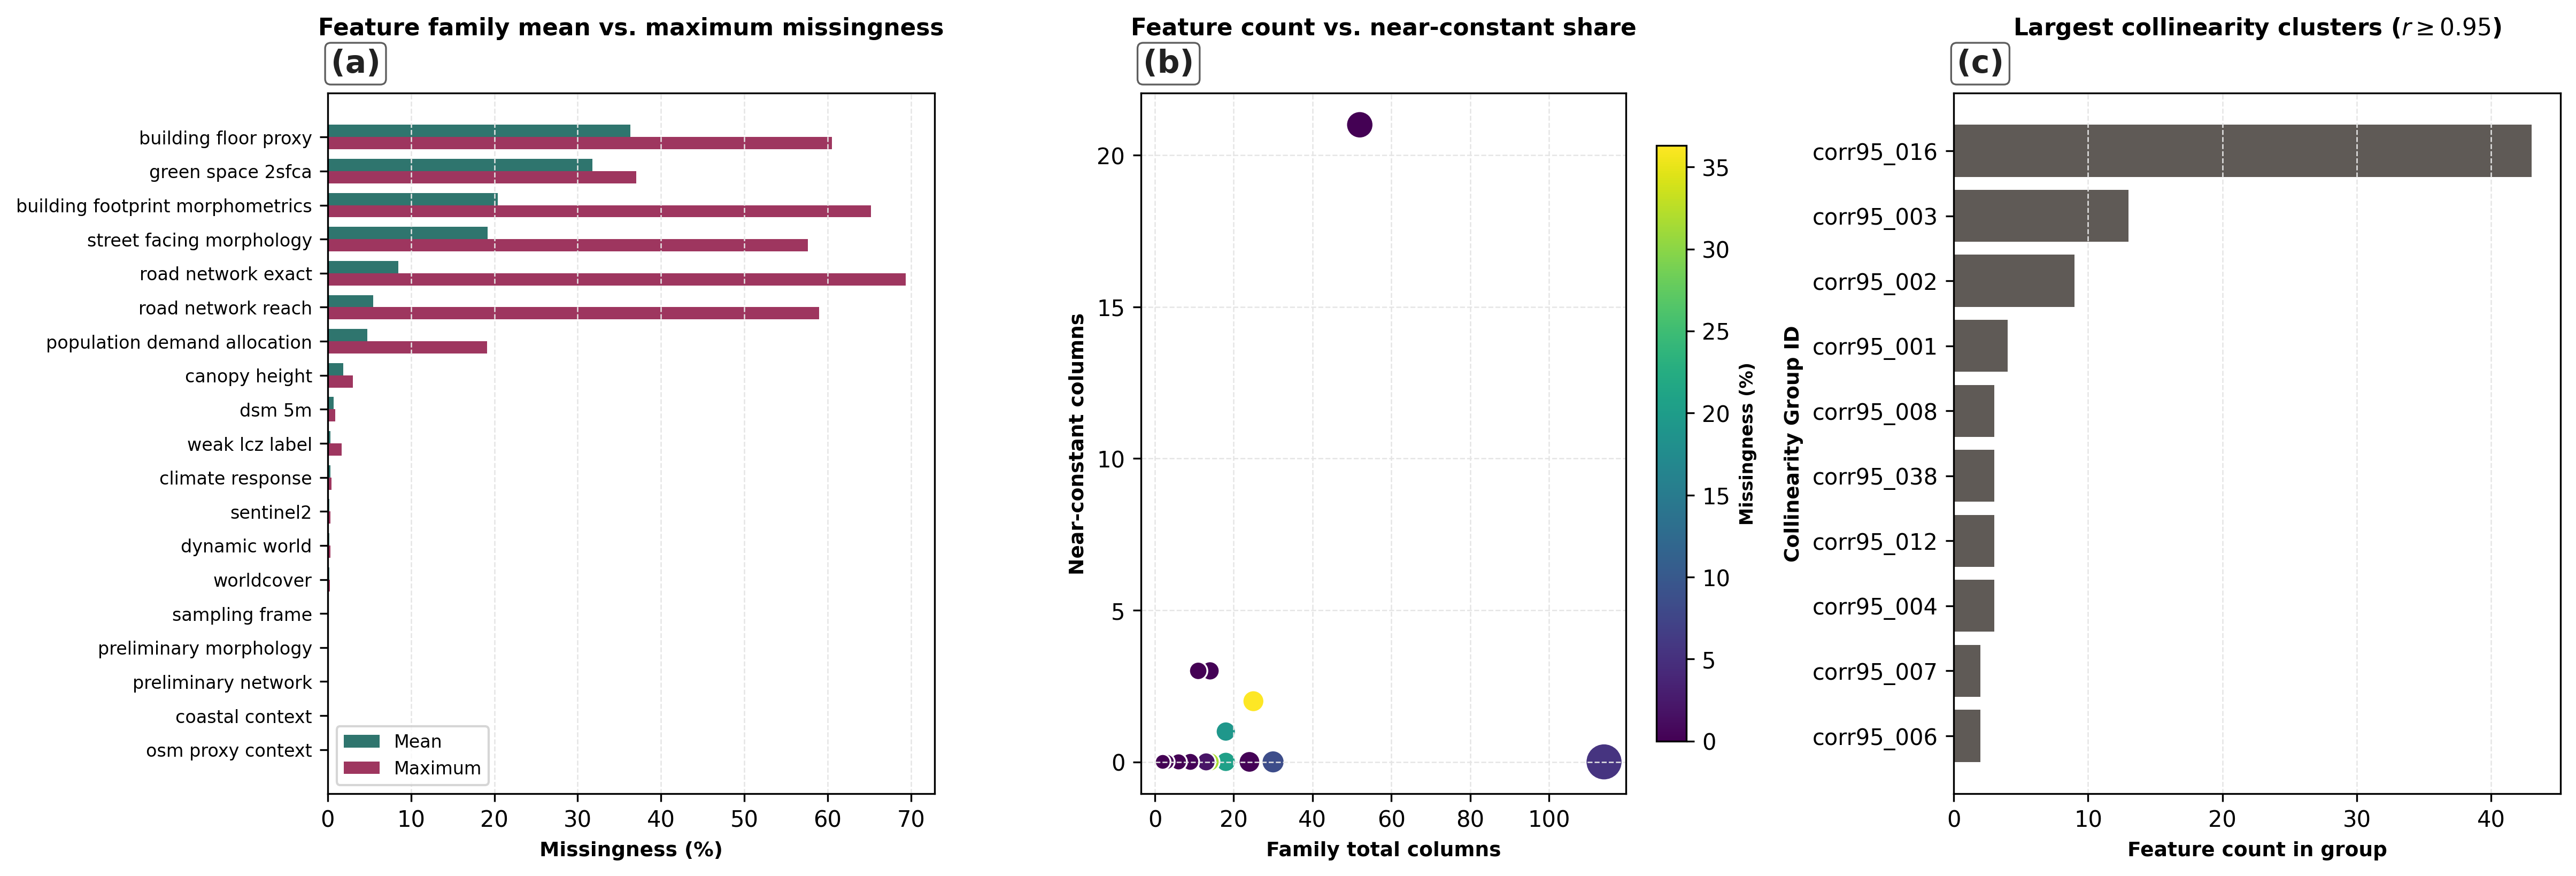
\includegraphics[width=0.96\textwidth]{fig_s2_feature_quality.png}
    \caption{Feature-quality diagnostic. (a) Mean and maximum missingness by
    family, (b) feature count versus near-constant columns, and (c) the largest
    high-correlation feature groups.}
    \label{fig:s2-feature-quality}
\end{figure*}
\FloatBarrier

\subsection*{S3. Spatial-fold diagnostics}

The primary spatial folds are fixed before model comparison. This diagnostic
shows class support by fold and the fold-wise distribution of the primary
LightGBM out-of-fold prediction probability. It is a stability diagnostic for
the weak-label baseline and does not constitute audited subtype validation.

\begin{figure*}[p]
    \centering
    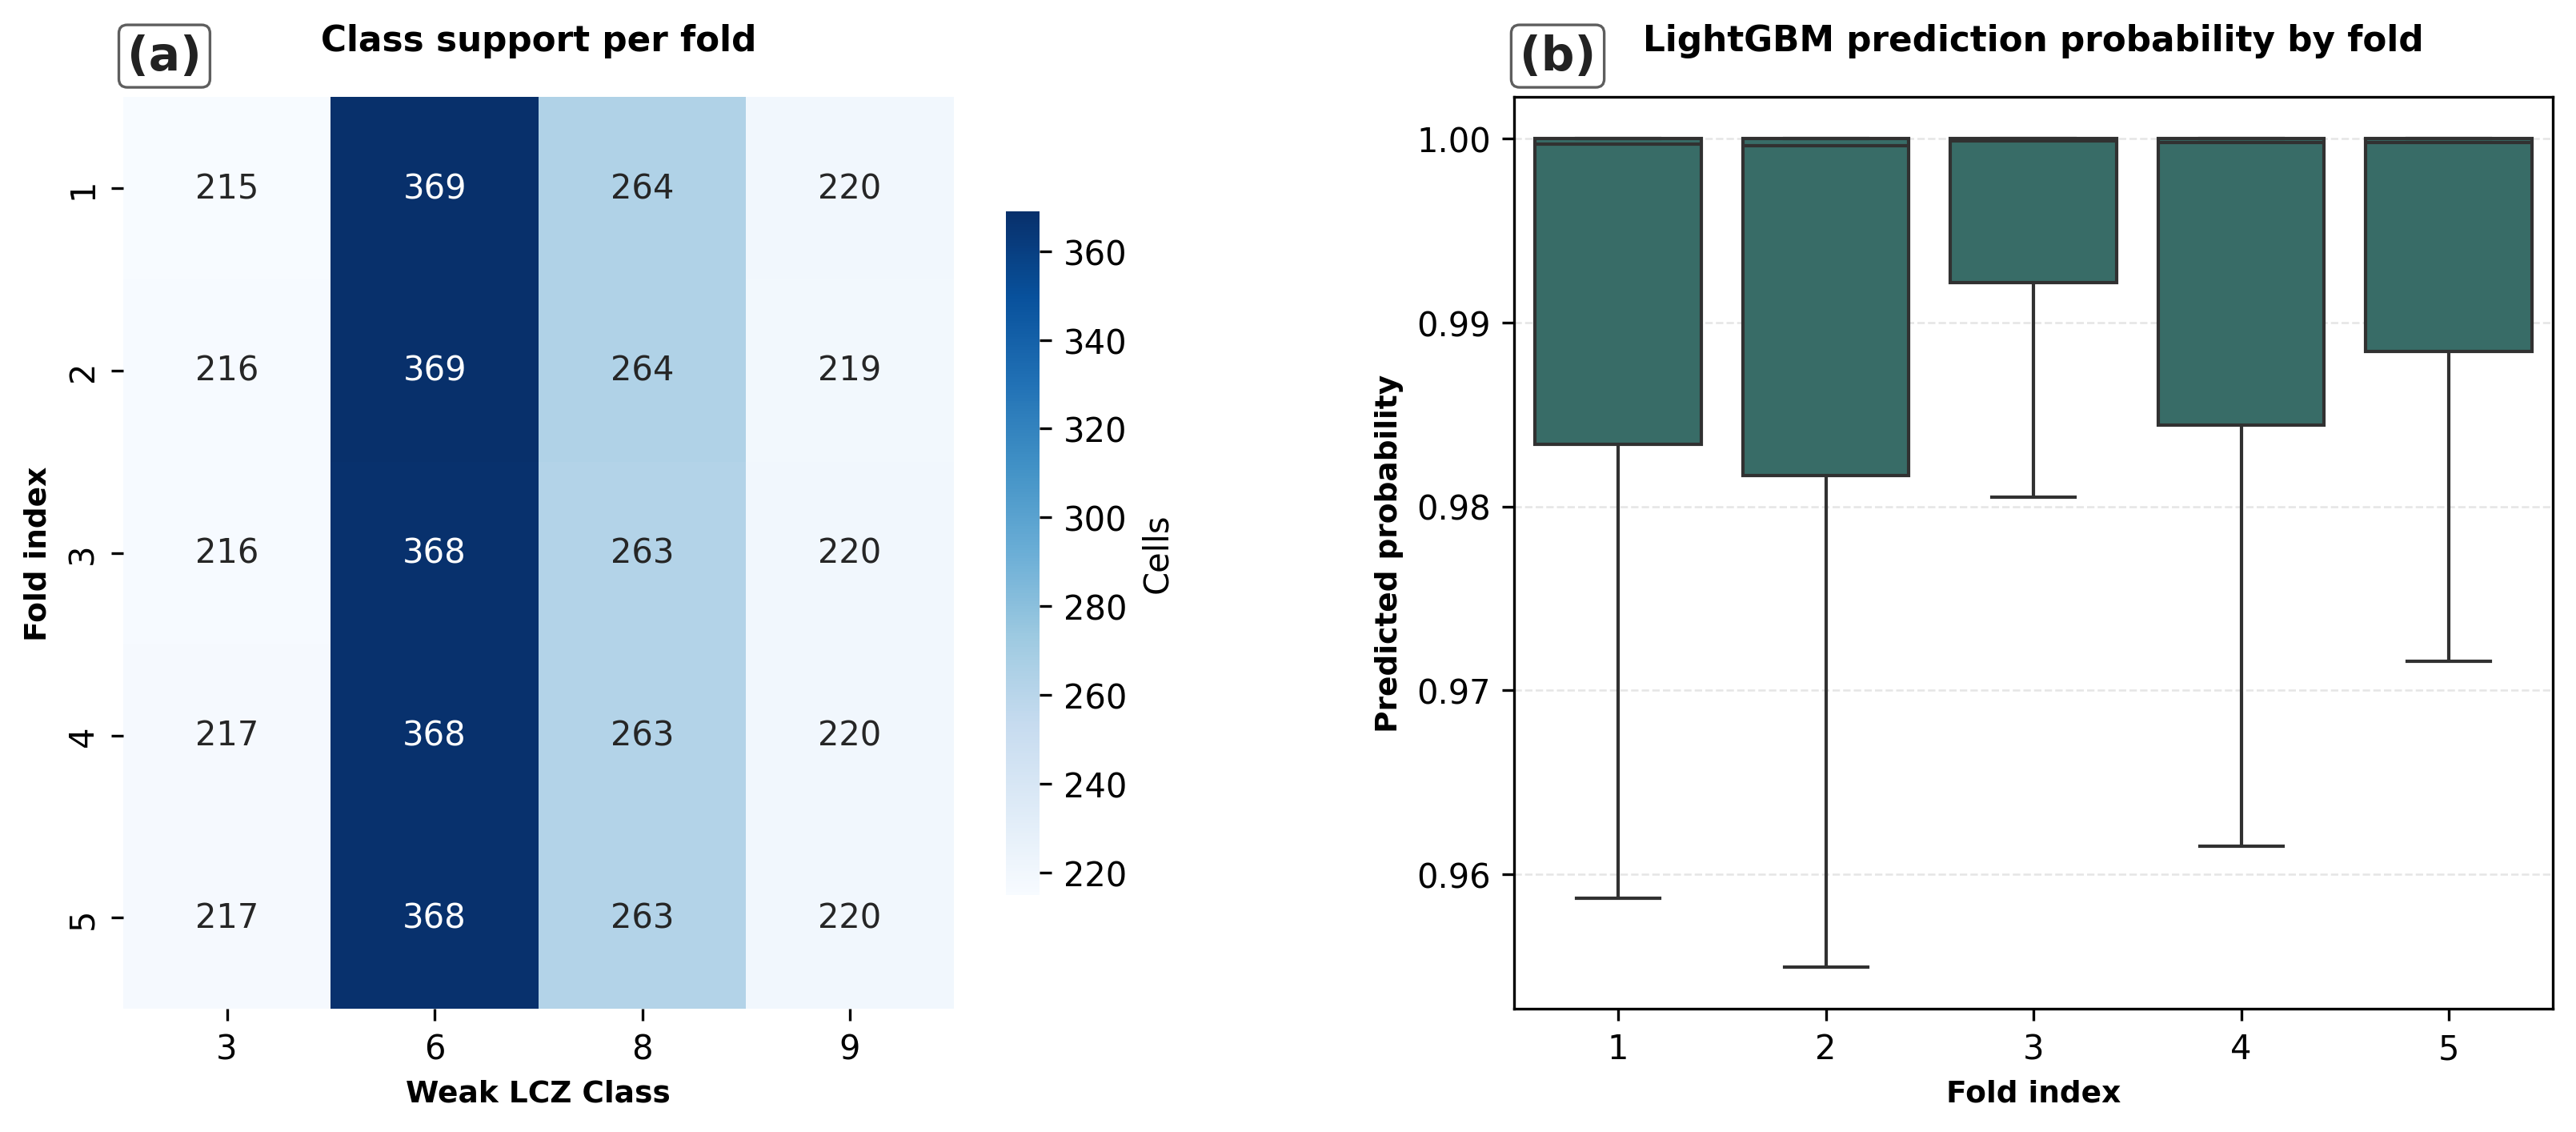
\includegraphics[width=0.92\textwidth]{fig_s3_spatial_fold_diagnostics.png}
    \caption{Spatial-fold diagnostics. (a) Weak-class support across the fixed
    spatial folds and (b) primary LightGBM out-of-fold prediction probability
    by fold.}
    \label{fig:s3-spatial-folds}
\end{figure*}
\FloatBarrier

\section*{Reproducibility and claim boundary}

The supplement is considered internally reproducible when the v8 input retains
16,506 rows and 374 fields, all manifest-referenced fields exist, the four-class
filter returns 5,339 rows, every eligible row has one spatial fold, preprocessing
is fitted inside training folds, and all reported out-of-fold outputs are
regenerated from the locked scripts and parameters. Manual audit and deep
multimodal fusion remain unavailable until their output manifests exist; no
supplementary panel here should be read as evidence that those gates have
already been passed.

\end{document}
